\documentclass[12pt]{article}

\usepackage{ctex}
\usepackage{geometry}
\usepackage{enumerate}
\usepackage{amsmath}
\usepackage{float}
\usepackage{subfigure} 
\usepackage{listings}
\usepackage{xcolor}
\usepackage{cases}
\usepackage{amssymb}    %triangleeq
\usepackage{lastpage}   %页码
\usepackage{fancyhdr}   %页眉页脚
\usepackage{graphicx}   %图片引用路径
\usepackage{indentfirst}    %缩进设置
\usepackage{booktabs}
\usepackage{multirow}
\usepackage{diagbox}

\setlength{\parindent}{2em}%缩进设置
\graphicspath{{C:/Users/adm/Desktop/课程文件/科学计算/作业/3.9作业/tex/image}}%图片引用Path,好像并没有什么用

%New colors defined below
\definecolor{codegreen}{rgb}{0,0.6,0}
\definecolor{codegray}{rgb}{0.5,0.5,0.5}
\definecolor{codepurple}{rgb}{0.58,0,0.82}
\definecolor{backcolour}{rgb}{0.95,0.95,0.92}

%Code listing style named "mystyle"
\lstdefinestyle{mystyle}{
  backgroundcolor=\color{backcolour},   commentstyle=\color{codegreen},
  keywordstyle=\color{magenta},
  numberstyle=\tiny\color{codegray},
  stringstyle=\color{codepurple},
  basicstyle=\ttfamily\footnotesize,
  breakatwhitespace=false,         
  breaklines=true,                 
  captionpos=b,                    
  keepspaces=true,                 
  numbers=left,                    
  numbersep=5pt,                  
  showspaces=false,                
  showstringspaces=false,
  showtabs=false,                  
  tabsize=2
}

%"mystyle" code listing set
\lstset{style=mystyle}
\usepackage{indentfirst}
\setlength{\parindent}{2em}%缩进设置

\graphicspath{{images/}}%图片引用Path
\geometry{left=1in,right=0.75in,top=1in,bottom=1in}     %页边距


\lhead{} %左上页眉

\begin{document}
\pagestyle{fancy}
\setcounter{page}{1}
\rhead{Page \thepage\ of \pageref{LastPage}}
%页码设置
\vspace{20pt}
\centerline{{\Large \textbf{计算机模拟 Homework 5}}}
\vspace{15pt}

\centerline{{\large \textbf{汪奕晨 3180105843}}}
\vspace{15pt}

\centerline{{\large \textbf{数学科学学院 数学与应用数学专业}}}
\vspace{15pt}

%============================== Q1 =========================================
%============================= Problem Restatement =============================
\section{问题描述}
我们知道三维格点的布朗运动是非常返的。

本文通过数值模拟计算返回概率。空间为$(x_i, y_i, z_i)$,其中$x_i, y_i, z_i$均为整数。初始位置为原点。每一步布朗运动,都等概地向上、下、左、右、前和后移动一格。
%============================= Theory and Algorithms =============================
\section{设计思路}
\subsection{实验设计思路}
同时考虑$S$个初始位于原点的点,独立抽取在三维空间中游走,各自进行$N$步,同时记录是否曾回到原点,可以得到$N$步后曾回到原点的比例$p$。

在实现的过程中,还可以记录每一步时的比例$p(N)$,绘制$p(N)-N$的图像。在一个实例(即$S$个点)中,$p(N)$关于$N$是严格单调递增的,这可能会使得结果存在偶然因素。故我们设置$M$个实例后取$p$的均值,来判断$p(N)$关于$N$的收敛情况


\subsection{代码设计思路}
这里给出一些代码设计的技巧

快速一次性抽取给定步数的运动结果。

可以使用np.random.choice快速抽取,使用逻辑索引对需要对$x,y,z$坐标进行$+1$或$-1$操作处向量化处理,而后使用np.cumsum方法快速获得累计值,即累计运动的偏移量,再加上当前的位置,既可以得到每一步运动后所处的位置。
\begin{lstlisting}[language = Python]
  walk = np.random.choice(np.arange(6), steps, True)
  new_path = np.zeros((3,steps))
  new_path[0][walk==0] += 1
  new_path[0][walk==1] -= 1
  new_path[1][walk==2] += 1
  new_path[1][walk==3] -= 1
  new_path[2][walk==4] += 1
  new_path[2][walk==5] -= 1
  new_path = np.cumsum(new_path, axis=1) + self.position.reshape(3,1)
\end{lstlisting}

快速生成latex表格,当不同参数的运行结果存在pd.DataFrame中时,可以使用df.to\_latex快速生成latex代码
\begin{lstlisting}[language = Python]
  with open('df_latex.txt','w') as tf:
    tf.write(df.to_latex())
\end{lstlisting}

%============================= Results =============================
\section{模拟结果与分析}
固定$M=20$,对不同规模的$S,N$求解,得到的结果如Table (\ref{tab: 1}),不同参数下$p(N)$随$N$的变化图如Figure (\ref{pic: perf})
\begin{table}[H]
  \centering
  % \diagbox[width=5em,trim=l]{$S$}{$N$}
  \begin{tabular}{lrrrrr}
    \toprule
    \diagbox[width=3em,trim=l]{$S$}{$N$} &      400  &      800  &      1200 &      1600 &      2000 \\
    \midrule
    50  &  0.307000 &  0.311000 &  0.313000 &  0.313000 &  0.313000 \\
    100 &  0.312500 &  0.315000 &  0.315500 &  0.317500 &  0.318000 \\
    150 &  0.332667 &  0.336667 &  0.338333 &  0.339667 &  0.340667 \\
    200 &  0.334500 &  0.339250 &  0.341500 &  0.342750 &  0.343500 \\
    \bottomrule
  \end{tabular}    
    
  \label{tab: 1}
  \caption{Results Table $M=10$}
\end{table}


\begin{figure}[H]
  \centering
  \subfigure[$S=100,N=2000,M=20$ $p-N$ Graph]{
  \begin{minipage}[t]{0.4\linewidth}
  \centering
  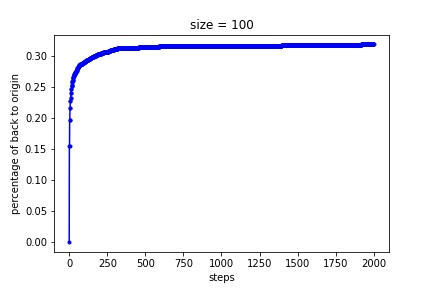
\includegraphics[width=7.5cm]{../rand_move_100_2000_20.jpg}
  \label{pic: perf 1}
  \end{minipage}
  }
  \subfigure[$S=200,N=2000,M=20$ $p-N$ Graph]{
  \begin{minipage}[t]{0.4\linewidth}
  \centering
  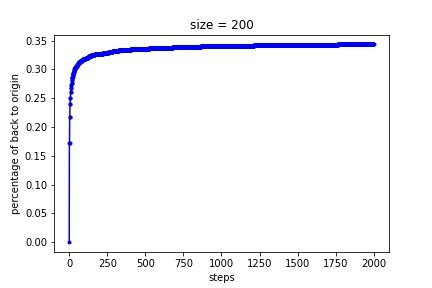
\includegraphics[width=7.5cm]{../rand_move_200_2000_20.jpg}
  \label{pic: perf 2}
  \end{minipage}
  }
  \caption{Performance of Simulation}
  \label{pic: perf}
\end{figure}

可以看到,随着$N$增大,$p$会收敛到$0.34$左右的数值, 且$S$越大,收敛地越快。







% %============================= Conclution and Disscusion =============================
% \section{结论与进一步工作}


% %============================== Reference =====================================
% \addcontentsline{toc}{section}{References}

% \begin{thebibliography}{99}
%   %\bibliographystyle{unsrt}
%   % \bibliographystyle{unsrt}
%   \bibitem{Ref1}%temperature map
%   Global Climate Change: Evidence. (2019, October 24). Retrieved January 16, 2020, from https://neo.sci.gsfc.nasa.gov/view.php?datasetId=MYD28M
  
% \end{thebibliography}

% % \nocite{*}
% % \bibliographystyle{acm}
% % \bibliography{test}
%================================ Appendix ========================================
\newpage
\section*{附录}
%============================= Codes =============================
\subsection*{代码}

\begin{lstlisting}[language=Python, caption = 随机游走类与批量游走类]
  import numpy as np
  import matplotlib.pyplot as plt
  from mpl_toolkits.mplot3d import Axes3D
  import time
  import pandas as pd

  class rand_move_3d():
    def __init__(self):
        self.position = np.array([0,0,0])
        self.path = self.position.reshape(3,1)
        self.step = 0
        self.back = np.array([])

    def rand_walk(self, steps):
        walk = np.random.choice(np.arange(6), steps, True)
        new_path = np.zeros((3,steps))
        new_path[0][walk==0] += 1
        new_path[0][walk==1] -= 1
        new_path[1][walk==2] += 1
        new_path[1][walk==3] -= 1
        new_path[2][walk==4] += 1
        new_path[2][walk==5] -= 1
        new_path = np.cumsum(new_path, axis=1) + self.position.reshape(3,1)
        
        self.path = np.hstack((self.path, new_path))
        self.position = self.path[:,-1]
        self.step += steps
        new_back = np.zeros(steps)

        if self.back.shape[0] > 0 and self.back[-1] == 1:
            new_back = 1
        else:
            origin = np.array([0,0,0])
            for i in range(self.step):
                if ( self.path[:, i+1] == origin ).all():
                    new_back[i:] = 1
                    break

        self.back = np.hstack((self.back, new_back))


    def plot_path(self, savepath=None):
        fig = plt.figure()
        ax = Axes3D(fig)

        ax.plot(self.path[0], self.path[1], self.path[2], 'b.-')
        if savepath:
            fig.savefig(savepath)
        fig.show()


  class batch_walk():
    def __init__(self, size):
        self.size = size
        self.persons = [rand_move_3d() for i in range(size)] if size else None

    def test(self, N):
        '''
        N: the number of steps
        '''
        self.n = N
        self.p = np.zeros(N)
        count = np.zeros(N)
        start_time = time.time()
        for i in range(self.size):
            self.persons[i].rand_walk(N)
            count += self.persons[i].back

        self.p = count/self.size
        end_time = time.time()
        # print('run time = {}'.format(end_time - start_time))
        # print('final percentage = {:.3f}'.format(self.p[-1]))
        return self.p
                
    
    def plot_p(self, p=None, savepath=None):
        plt.figure()
        x = np.arange(self.n)
        if p is None:
            p = self.p
        plt.plot(x, p, 'b.-')
        plt.xlabel('steps')
        plt.ylabel('percentage of back to origin')
        plt.title('size = {:}'.format(self.size))
        if savepath:
            plt.savefig(savepath)
        plt.show()
\end{lstlisting}

\begin{lstlisting}[language = python, caption = 测试模块]
  def para_test(size, step, N):
    p = np.zeros(step)
    for _ in range(N):
        B = batch_walk(size)
        p += B.test(step)
    p /= N
    B.plot_p(p=p, savepath='rand_move_{:}_{:}_{:}.jpg'.format(size,step,N))
    return p

  def paras_test(size_list, step_list, N):
    df = pd.DataFrame(np.zeros((len(size_list), len(step_list))))
    for i,size in enumerate(size_list):
        # for N in N_list:
        p = para_test(size, step_list[-1], N)
        df.loc[i,:] = p[step_list-1]
        print('size = {} is done'.format(size))
    df.index = size_list
    df.columns = step_list
    return df

  size_list  = np.array([50*i for i in range(1, 5)])
  step_list = np.array([400 * i for i in range(1, 6)])
  N = 10

  df = paras_test(size_list, step_list, N)
  with open('df_latex.txt','w') as tf:
    tf.write(df.to_latex())
\end{lstlisting}
\end{document}